\chapter{Theory}

\begin{chapterabstract}
This chapter outlines the theoretical basis for both the concepts and measurements relevant to this thesis. We start with very brief overview of Fermi liquid theory, leading on to the theory behind the \ac{dHvA} torque technique, then a brief overview of \ac{DFT} and magnetotransport.
\end{chapterabstract}



\section{Fermi liquid theory}

The nearly-free electron gas model for ordinary metals\footnote{A model which only considers the kinetic energies of the electrons and Pauli exclusion terms} is an extremely coarse approximation to the real situation and yet provides surpringly good, predictive results in a variety of scenarios. Fermi liquid theory provides the theoretical basis which explains why we can use non-interacting particle models with a simple modification of the masses of the interacting Fermionic particles.

From a matchematical standpoint, Fermi liquid theory considers a gas of non-interacting particles and gradually `switches on' the interactions. Provided the system transitions adiabatically\footnote{i.e. with no symmetry breaking changes in phase or, in other words, there is a one-to-one mapping of the particles in the initial non-interacting system to the quasiparticles in the final interacting system} then the `particles' in the resulting system, which is known as a \emph{Fermi liquid}, can be modeled using the same mathematics as the non-interacting system with an adjusted mass. This adjusted mass is known as the \emph{enhanced mass} and encompasses the interactions in the system with the magnitude being an indicator of the interaction strength. The enhanced mass particles are labeled quasiparticles since they no longer share the same mass as an electron at rest and are, arguably, a product of a mathematical abstraction.

At the time of writing, Fermi liquid theory describes what would be considered `ordinary' metals with deviations from Fermi liquid theory generally considered of interest in a number of systems. Moreover the theory behind measurement techniques such as \ac{dHvA} --- decribed in the next section --- rely on the existence of coherent quasiparticles at the Fermi surface to be valid. The reconscilliation of observed \ac{dHvA} oscillations in cuprates with evidence for reduced quasiparticle weight from \ac{ARPES} data currently provides one of the interesting challenges of \highTc research.



\section{De Haas-va Alphen oscillation}

In this section the phenomenon of \ac{dHvA} oscillations is described. It is not immediately apparent how a ramping magnetic field could cause oscillations in such a wide range of parameters but Lifshitz and Kosevich established their eponymous equation based on a theoretical basis set out by Landau which was then used to characterise the Fermi surface of many metals and establish the field of `Fermiology'. Strictly, only the oscillations in magnetisation are \ac{dHvA} oscillations and those in resistance are called Shubnikov-de Haas oscillations. Nonetheless they both originate from the same underlying phenomena of oscillations in the system energy.

\subsection{Overview}

For metals, the majority of the interesting physics occurs at the Fermi level and, provided Fermi liquid theory holds true, the electrons at the Fermi level can be modelled to a high degree of accuracy with the Sommerfeld model --- that is a Fermi gas of non-interacting electrons in an infinite box. When a magnetic field is applied, the electrons have their usual grid pattern distribution of plane wave k-vectors rearranged such that the electrons move around orbital and helical paths. These rearranged k-vectors form a set of concentric tubes, known as Landau tubes, whose cross-sectional area, $a$, perpedicular to the field is given by the Onsager relation:\footnote{Derivations of the Onsager relation are given in several textbooks including pg. 32 of Schoenberg\cite{Schoenberg1984} and pg. 272 of Ashcroft \& Mermin\cite{Ashcroft1976}.} 
%%
\begin{equation}
\label{Eqn:Theo:Onsager}
\textit{a}_{k_{\perp}} = (r + 1/2)\frac{2\pi e B}{\hbar}
\end{equation}
%%
where $r$ is a quantisation number that sets apart each tube. We can see from the relation that as $\vect{B}$ increases, so does the cross-sectional area of the tubes. As the magnetic field is ramped, successive tubes periodically pass the Fermi surface causing a spike in the \ac{DOS} at the Fermi level and also oscillations in the energy o the ssytem, $E$, which, for geometric reasons explained in the next section, are far stronger at the maximumal and minimal (extremal) areas of Fermi surface. Thermodynamic quantities such as magnetic susceptibility ($\chi = \partial E/\partial B$) and heat capacity ($C_{V} = \partial^2E/\partial T^2|_{V}$) or quantities that depend on the \ac{DOS} at the Fermi level such as electrical resistance all oscillate as the field is ramped. Oscillations in the susceptibility are known as \ac{dHvA} oscillations, oscillations in the resistivity are known as Shubnikov-de Haas oscillations.

 We can relate the `frequency' $F$ (measured in $tesla$\footnote{n.b. that it is \textit{tesla} and not \textit{tesla$^{-1}$} because, as we shall see later, the oscillations are actually periodic in $1/B$ and \textit{not} $B$ so their frequency counterpart is measured in \textit{tesla}.}) that the tubes pass the Fermi surface to the extremal Fermi surface area using the following application of the Onsager relation,
%%
\begin{equation}
\textit{a}_{k_{\perp}} = \frac{2\pi e }{\hbar}F
\end{equation}
%%
By varying the direction of the field we can obtain a series of maximal and minimal Fermi surface areas in a variety of orientations in order to build a profile of the Fermi surface topology and size. In practice, there are many possible variations that might fit the model based on areas of cross-sectional slices alone and so typically ab-initio \ac{DFT} calculations --- described in sections~\ref{Sec:Theo:Dft} and~\ref{Sec:Exp:Dft} --- are employed to provide a basis which can be tweaked based on the constraints from the measurements. 

A more detailed analysis of this process follows, beginning with an illustrative mathematical treatment for oscillations in the magnetisation.

\subsection{Exploring the origin of the oscillations}

We begin by calculating the degeneracy of the Landau tubes i.e. the number of electron states per tube. Because the states under a magnetic field are a one-to-one rearrangement of the states with no field, we can use the Sommerfeld number of states per unit k-space ($V/4\pi^3$) to determine the degeneracy. From the Onsager relation (eqn.\ref{Eqn:Theo:Onsager}) we see that the additional area for successive tubes is $\Delta a_{k_{\perp}}  = 2\pi e B/\hbar$ which we can convert to a volume by integrating over $k_{\perp}$. This gives a degeneracy per tube therefore of,

\begin{equation}
D_{\textrm{tube}} = d k_{\perp}\left(\frac{2\pi e B}{\hbar}\right)\left(\frac{V}{4 \pi^3}\right) = \frac{eBVdk_{\perp}}{\hbar 2\pi^2}
\end{equation}

We continue by writing an expression for the energy of the system, $E$ by summing the energies of the states that lie beneath the cross-sectional area defined by the Fermi surface ($a_{k_\perp F}$) for a given $k_\perp$. To do this, we use the Onsager equation to determine $R_\perp$ --- the number of Landau tubes below the Fermi surface at this cross-sectional slice. We then multiply this by the degeneracy of the tubes, $D$ and the energy for states on that particular Landau tube, $\epsilon_r$,
%%
\begin{equation}
\label{Eqn:Theo:OscillateE}
E = D\sum_{r}^{R_\perp}\epsilon_r = \frac{eBVdk_\perp}{\hbar 2 \pi^2}\sum_{r}^{R_\perp}\epsilon_r
\end{equation}
 where,
\begin{equation}
R_\perp = \textrm{floor}\left[\frac{a_{k_\perp F}\hbar}{2\pi e B} - \frac{1}{2}\right]
\end{equation}
%%
To complete the above equation, we need an expression for the energies of each of the Landau tubes. The procedure for the free electron case is to insert the canonical momentum (i.e momentum of a free electron in a magnetic field) into the non-interacting Schr\"odinger equation and solve to obtain the following eigenvalues for the energies on the Landau tubes. Full derivations can be found in several textbooks\footnote{See for examples pg. 32ff. in Schoenberg\cite{Schoenberg1984} or pg. 148ff. in Blundell\cite{Blundell2001}.} and so will  not be repeated here. Below is the expression for the energy eigenvalues,
%%
\begin{equation}
\epsilon_r=(r+1/2) \hbar \omega_c + \frac{\hbar^2 k^2}{2m_0} \textrm{\hspace{0.2cm}where,\hspace{0.2cm}} \omega_c = \frac{eB}{m_0}
\end{equation}
%%
and is known as the \textit{cyclotron frequency}. The summation term in equation\ref{Eqn:Theo:OscillateE} can now be written,
%%
\begin{align*}
\sum_r^{R_\perp}\epsilon_r &= \sum_r^{R_\perp}\left( (r+1/2) \hbar \omega_c + \frac{\hbar^2 k^2}{2m_0} \right) \\
    &= \frac{\hbar eB}{m_0}\sum_r^{R_\perp}r + \frac{\hbar eB}{2m_0}\sum_r^{R_\perp}1 + \frac{\hbar^2 k^2}{2m_0}\sum_r^{R_\perp}1 \\
    &= \frac{\hbar eB}{2 m_0} R_\perp(R_\perp + 1) + \frac{\hbar eB}{2m_0}R_\perp + \frac{\hbar^2 k^2}{2m_0}R_\perp \\
    &= \frac{\hbar eB}{2m_0}R_\perp^2 + \left(\frac{\hbar eB}{m_0} + \frac{\hbar^2 k^2}{2m_0}\right)R_\perp
\end{align*}
%%
which can be expanded out and finally substituted back into equation\ref{Eqn:Theo:OscillateE} to finally obtain,
%%
\begin{equation}
\label{Eqn:Theo:OscIllustration}
E = \frac{e^2Vdk_\perp}{4\pi^2m_0}B^2\left[R_\perp^2 + 2R_\perp + \frac{\hbar k^2}{e}\frac{1}{B}R_\perp\right]
\end{equation}
%%
Key to the above relation is that, although $R_\perp$ is inversely proprtional to $B$, it remains discrete. This gives rise to the saw-tooth like function shown in figure~\ref{Fig:Theo:EnergyOscillations} for some typical experimental parameters. Also plotted is the fuction against $1/B$ where we can clearly see that the oscillations are periodic in inverse field hence the frequency being measured in tesla$^{-1}$.
%%
\begin{figure}[htbp]
    \begin{center}
        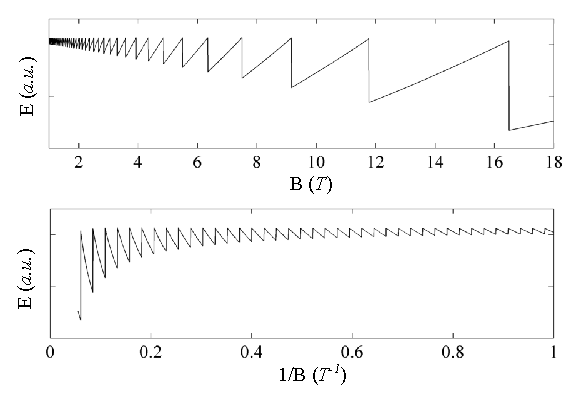
\includegraphics[scale=0.9]{Chapter-Theory/Figures/TheoreticalOscillations/TheoreticalOscillations}
        \caption{Theoretical energy oscillations for a Fermi surface orbit which is 5\% of a \unit{5}{\angstrom} cubic \ac{BZ} between \unit{1-18}{\tesla}. Kinetic energy term is taken to be for an electron at a level half the size of the Fermi surface.}
        \label{Fig:Theo:EnergyOscillations}
    \end{center}
\end{figure}

The above is not a rigourous derivation but is nonetheless illustrative of the origin of the oscillation in the system energy and how any thermodynamic value which depends on the energy of the system oscillates as a function of field. To continue we need to include correction factors to the oscillation amplitude due to finite electron scattering rates ($A_D$), temperature ($A_T$), Zeeman splitting of spins ($A_s$), doping ($A_{\textrm{dop}}$), mosaicity ($A_{\textrm{mos}}$), warping of the Fermi surface ($A_{\textrm{warp}}$) as well as adjustments due to the fact that the parameter measured was torque of the sample in a field and not the energy or magnetisation directly ($A_{\Gamma}$). For this, we turn to a more solid foundation that was put forward by Lifschitz and Kosevitch and presented by Schoenberg.

\subsection{\acl{LK} equation}

The derivation for the full expression for the Landau thermodynamic potential, $\Omega$\footnote{Formally defined as the energy in a open system that is in thermal contact with its surroundings}, begins in a similar way to the previous illustrative example but frames the sawtooth-like function above as a more mathematically manageable Fourier decomposition which also conveniently makes the technique highly amenable to Fourier analysis. For this reason the equation below features higher harmonics which are denoted with the identifier $p$.
%%
\begin{equation}
\Omega = \left(\frac{e}{2\pi\hbar}\right)^{\frac{3}{2}}\frac{e\hbar B^{\frac{5}{2}}}{m_0 \pi^2}\left| \frac{\partial^2 a_{\textrm{ext}}}{\partial k^2_\perp}\right|^{-\frac{1}{2}}\sum_{p=1}^{\infty}p^{-\frac{5}{2}}A_{\textrm{tot}}\cos\left[2\pi p\left(\frac{F}{B} - \gamma\right)\pm\frac{\pi}{4}\right]
\end{equation}
where,
\begin{equation}
A_{\textrm{tot}} = A_T A_D A_s A_{\Gamma} A_{\textrm{mos}} A_{\textrm{dop}} A_{\Delta B}
\end{equation}
%%
The above equation and derivatives of it are known as the \ac{LK} equation. To obatin the magnetisation the differential with respect to $b$ is taken to get,
%%
\begin{equation}
M = \left(\frac{e}{\hbar}\right)^{\frac{3}{2}}\frac{e\hbar F V B^{\frac{1}{2}}}{m_0 \pi^\frac{5}{2}\sqrt{2}}\left| \frac{\partial^2 a_{\textrm{ext}}}{\partial k^2_\perp}\right|^{-\frac{1}{2}}\sum_{p=1}^{\infty}p^{-\frac{3}{2}}A_{\textrm{tot}}\sin\left[2\pi p\left(\frac{F}{B} - \gamma\right)\pm\frac{\pi}{4}\right]
\end{equation}
%%
To attain the above equations, it was necessary to perform an integral over $k_\perp$\footnote{Similar to the integral in the toy equation from the previous section} which results in a parameter for an extremal Fermi surface orbit area perpendicular to the field given by $a_{\textrm{ext}}$. 

\subsubsection{Attenuation for non-extremal orbits}

Only the extremal (i.e. the largest and smallest) magnetically induced orbits contribute significantly to oscillations in the system energy. This is because $F$ represents a phase factor in the \ac{LK} equation and at the extremal points $dF/dk_\perp=0$ meaning more orbits near extrema are in phase. However it is not immediately clear how much stronger the oscillations from the extremal orbits will be in comparison to other orbits. Figure~\ref{Fig:Theo:ExtremalPhases} shows examples of the strengths of the oscillations after integrating over a distribution of phases shown in the insets.
%%
\begin{figure}[htbp]
    \begin{center}
        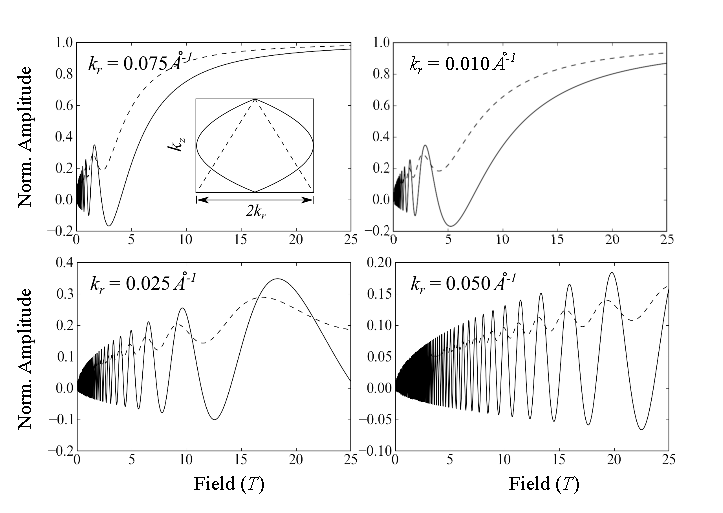
\includegraphics[scale=0.8]{Chapter-Theory/Figures/ExtremalPhases/ExtremalPhases}
        \caption{The sum of 1000 cosines with phase dispersions shown in the insets. Dashed line represents an extremal dispersion, solid lines a spread of linear dispersions and dotted line represent a non-extremal inflection point. Top left, top right and bottom left panels have phase distributions that are scaled from $0$ to $\sim1$, $\approx10$ and $\approx100$ Landau tube `wavelengths' respectively.}
        \label{Fig:Theo:ExtremalPhases}
    \end{center}
\end{figure}
%%
The panels each show the phases from the distributions taken over a range of scales, and it is clear that the phase cancellation is more acute for longer scales. This makes sense if we consider that the Landau tubes passing the Fermi surface are a oscillatory measurement probe like any other and so will be wavelength limited. That is, if the difference between the outermost and innermost orbits are of the order of the Landau tube spacing as is passes the Fermi surface, then the oscillations will be difficult to pick out. Interestingly this also places a limit on the maximum field that can be used to probe a Fermi surface since, according to the Onsager relation, the larger the field the larger the spacing between tubes. In practice this is simply $\Delta a_{k_\perp}$ which means that in terms of $F$, the resolutions is simply the field (i.e. $\sigma_F \sim \unit{18}{\tesla}$ for the Yellow magnet at Bristol). 

A final point is that it is not strictly extremal points that contribute significantly to the oscillations, but also inflected stationary points as shown in the last panel of figure~\ref{Fig:Theo:ExtremalPhases} so on could imagine a pathological stepped Fermi surface that would feature several strong orbital oscillations which would not be at turning points.

Variations in the phases can also be put into practice to model the various effects on the \ac{LK} equation listed towards the end of the previous section. These can be manifest by convolving an appropriate phase distribution function with the cosine oscillatory term. It can be shown\footnote{See for example, Schoenberg pg 57--59.\cite{Schoenberg1984}} that this convolution results in a relatively simple multiplication factor --- hence the various $A$ factors listed in the \ac{LK} equation which we expand upon below.

\subsubsection{Attenuation due to temperature}

To find the appropriate phase distribution function for the temperature dependence we start with the Fermi distribution,
\begin{equation}
\label{Eqn:Theo:FermiFunction}
f(\epsilon) = \frac{1}{\exp\left((\epsilon-\mu)/kT\right) + 1}
\end{equation} 
The differential of this distribution results in the broadening function (which is proportional to the probability that the Fermi energy $\mu$ is between $\epsilon$ and $\epsilon + d\epsilon$),
\begin{equation}
  P(\epsilon < \mu < \epsilon + d\epsilon) \propto \frac{d\epsilon}{2kT(1 + \cosh[(\epsilon - \mu)/kT])}
\end{equation}
This is convolved across the Fermi energy to smear it and also the phase through the parameter $F$. The details of how this is done is given in Schoenberg pg. 59ff~\cite{Schoenberg1984} with the end result is given by,
\begin{equation}
\label{Eqn:Theo:TemperatureTerm}
  A_T = \frac{X}{\sinh(X)} \textrm{\hspace{0.3cm} where,\hspace{0.3cm}} X = \frac{2\pi^2pkT m^*_T}{e\hbar B}
\end{equation}

The above factor includes $m^*_T$, the \textit{thermal effective mass} as a term in a function of $T$. As a consequence, by studying the temperature dependence of the amplitude it is possible to get a measure of $m^*_T$ of the electrons at the extremal orbit. Techniques for doing this are discussed in section~\ref{Sec:Exp:ExtractingEffMassTemperatureDependence}.

The effective mass determined in this way is enhanced subject to the same interactions as in heat capacity experiments --- i.e. electron-phonon interactions and spin symmetric correlations --- but are probed for a particular Fermi surface orbit, whereas heat capacity is bulk averaged. As we will see later the mass enhancement is is different to that from spin measurements. For more one this see Rourke \etal\cite{Rourke2010b} and references therein.

\subsubsection{Attenuation due to finite quasiparticle lifetime}

The \textit{Dingle factor}, $A_D$, is due to the finite lifetime, $\tau$, of the electron quasiparticles due to scattering. Because of this time scale, there is a smearing of the electron energy through the uncertainty principle with a broadening which is approximately Lorentzian in shape. If we assume $\tau$ does not change with energy\footnote{This is not the case, but at most only a few Landau levels contribute to a particular oscillation and if we assume that the energy does not vary too much between subsequent levels then the assumption is a good one}, then this can be modeled as a smearing of the Fermi level such that the broadening function is,
\begin{equation}
  P(\epsilon < \mu < \epsilon + d\epsilon) \propto \frac{d\epsilon}{(\epsilon - \mu)^2 + (\hbar/2\tau)^2}
\end{equation}
and such that after the routine Fourier transform, the end relation is given by,
\begin{equation}
  A_D = e^{-\pi p m_b/e B\tau} = e^{-\pi p/\omega_c\tau} 
\label{Eqn:Theo:DingleTerm}
\end{equation}
The exponent in the above can be thought of as the number of orbits the electron has completed (i.e. each harmonic $p$ is another successive orbit) divided by the expected number of orbits it will complete, so evidently we expect to see the higher harmonics having an exponentially lower amplitude. The term $m_b$ refers to the \textit{band mass} which will be discussed in detail later on. 
%The mass term here is \TODO{How is it coupled as Tony described?}

\subsubsection{Attenuation due to spin splitting}

Applying a magnetic field causes a Zeeman splitting of energy levels of amgnitude,
\begin{equation}
  \Delta\epsilon = \frac{g e \hbar B}{2 m_e}
\end{equation}
where $m_e$ is the free electron mass and $g$ is a factor that is $\approx2$ for free electrons. Rather than smearing, this can be thought of as two separate Fermi surfaces with separate Fermi energies. The attentuation is given then as,
\begin{equation}
  A_s = \cos\left(\frac{\pi p g m^*_s}{2m_e}\right)
\end{equation}
where $m^*_s$ is the \textit{spin effective mass}. This is subject to a different set of interaction in comparison to the thermal effective mass -- notably both spin symmetric and antisymmetric correlations but not the electron-phonon interactions. As such, in materials with strong phonon interactions we may see a strong difference in $m^*_s$ and $m^*_T$.

\subsubsection{Other attenuating factors}

Another attenuating factor due to slight misalignments in the crystal structure, ($A_{mos}$), causing a mosaic polycrystalline structure could be modeled with an appropriate broadening function. Schoenberg suggests a Lorentzian similar to the Dingle factor --- there is no solid mathematical basis for this but no other function shape has been observed in experiment. The final form would then look like the following,
\begin{equation}
  A_{\textrm{mos}} = e^{2\pi p \Delta F_{\textrm{mos}}/B}
\end{equation}
where $\Delta F_{mos}$ is a parameter that determines the degree of overall misalignment.

The final attenuating factors mentioned here are $A_{\Delta B}$, the damping due to field inhomogeneity which has an effect depending on the shape of the field and $A_{\textrm{dop}}$, which is another Lorentzian-like broadening factor due to the doping inhomogeniety in the sample. Neither of which will be considered in the thesis --- the material studied is undoped, and the magnet is suitably large as to have an essentially linear field profile ---doping and so will not be explored further\footnote{If you do want to consider these factors, ref~\cite{Rourke2010b} has a passage on doping homogeneity and pg. 64 of Schoenberg discusses field inhomogeneity~\ref{Schoenberg1984}.}

\subsection{Zeeman-Doppler shifting of oscillations}

One ramification of the spin splitting is that as the field ramps there is a gradual increase and/or decrease in the size of the split Landau levels commensurate with field with $\Delta a \propto B$. In a paramagnetic material we expect there to be a majority of spins aligned with the field meaning the Fermi surface will mostly shrink as the field ramps in one direction and expand as it ramps in the opposite direction. This leads to an apparent extra shift in the frequency which is proportional to $B$ which is of order of the field strength.


\subsection{Band mass}

So far, three different electron masses have been defined, the thermal effective mass, the spin effective mass and the free electron mass. To tie these together a fourth mass is introduced, the \textit{band mass}. This is another effective mass resulting from the electrons being subject to the bandstructure potential as defined by \ac{DFT} calculations and is given by,
\begin{equation}
  m^*_b = \hbar^2 \left(\frac{d^2\epsilon}{dk^2}\right)^{-1} = \frac{\hbar^2}{2\pi}\frac{\partial a_{k_\perp}}{\partial \epsilon}
\end{equation}
Mass enhancement comes from any kind of interactions the electron has with its environment --- i.e. external fields, other electrons and nuclei --- resulting in the free electron mass $m_e$ becoming enhanced (renormalised). The bands mass can be determined from \ac{DFT} and the resulting enahcement is purely from the interaction of the electron with the calculated lattice potential. However \ac{DFT} calculations typically do not model correlation effects well or dynamic interactions at all. We know that both the thermal effective mass and the spin effective mass incorporate the band mass enhancements plus a unique set of interactions specified previously. Figure~\ref{Fig:Theo:EffectiveMassInheritance} lays out how the effective masses build on each other by incorporating more interactions.
\begin{figure}[htbp]
    \begin{center}
        \includegraphics[scale=0.9]{Chapter-Theory/Figures/EffectiveMassInheritance/EffectiveMassInheritance}
        \caption{A diagram showing how the succeessive electron masses build on the previous interactions. Additional interaction effects are listed in italics.}
        \label{Fig:Theo:EffectiveMassInheritance}
    \end{center}
\end{figure}
because of this particular hierarchy, it is sometimes possible to compare effective masses to get a sense of scale of the interactions.

\subsubsection{A 2D Approximation}

Although none of the attentuating factors above have an explicit angle dependence, they do vary as a function of angle through the band mass. A common approximation to simulate the dependancy in layered systems is to assume the Fermi surface is two dimensional in shape and therefore cylindrical. The cross section of a cylinder is given by,
\begin{equation}
    a = \frac{a_0}{\cos \theta},
\end{equation}
where $\theta$ is the angle from the cylinder axis. Increasing the Fermi energy by $\Delta \epsilon$ will cause the cross section at zero angle to change by amount $\Delta a_0$, then the band mass is given by,
\begin{equation}
    m^*_b = \frac{\hbar^2}{2\pi}\frac{\partial a_{k_\perp}}{\partial \epsilon} = \frac{\hbar^2}{2\pi}\frac{\partial}{\partial \epsilon}\left(\frac{a_0 + \Delta a_0 }{\cos\theta} - \frac{a_0 }{\cos\theta}\right) = \frac{\hbar^2}{2\pi}\frac{\partial a_0}{\partial \epsilon}\frac{1}{\cos \theta},
\end{equation}
therefore
\begin{equation}
    m^*_b = \frac{m^*_{b0} }{\cos{\theta}}
\end{equation}
This means that under this approximation, any factor that includes the band mass, explicitly or implicitly\footnote{Meaning $m^*_T$ and $m^*_S$ which are both enhancements of the band mass} can be resolved using the the zero angle band mass with an angle dependence of $1/\cos{\theta}$.

\subsection{Final theoretical observations}

Originally \ac{dHvA} measurements were used to measure the Fermi surfaces of elemental metals and so the initial assumption of a free-electron gas is justified based on the fact that elemental metals have a Fermi surface and are considered materials that adhere to Fermi liquid theory. The fact that oscillations have been observed in cuprates and pnictides which have demonstrated non-Fermi liquid behaviour is therefore remarkable and moreover implies the presence of a Fermi surface, at least in the prescence of a strong magnetic field.




\section{Spin density wave instability}
\label{Sec:Theo:SpinDensityWave}

Section~\ref{Sec:Intro:Nesting} discussed the possibility of high-$T_c$ pairing being due to fluctuations in close proximity to a \ac{SDW} state. Here we briefly describe the \ac{SDW} state and some of the theory behind it.

Broadly speaking a \ac{SDW} is a magnetic state just as ferromagnetism and antiferromagnetism are magnetic states. In its most general sense, a \ac{SDW} is a periodic modulation of magnetic spins in both space and time hence it being a `wave of spin density'. \ac{AFM} is actually a special case of a \ac{SDW} which does not vary in time, i.e. is static, and also varies spatially with the periodicity being some multiple of the real-space lattice vector, i.e. is commensurate with the lattice. Ferromagnetism can be thought of as a \ac{SDW} state with wavevector $\vect{q}=0$ i.e. it has no periodic variation and so is not really a `wave'.

Using the mean field \ac{HFA} the following expression gives the stability condition for the \ac{SDW} state~\cite{Moriya1985},
\begin{equation}
2I\chi_0(\vect{q}) > 1,
\end{equation}
where $I$ is the exchange energy between electron bands and $\chi_0$ is the Lindhard susceptibility. The greater the Lindhard susceptibility, the more stable the state.

\subsection{Lindhard susceptibility}
\label{Sec:Theo:Susceptibility}

The Lindhard susceptibility models the Stoner excitations (i.e. electron-hole scattering) of a nearly free electron system. To derive the Lindhard susceptibility, we begin with a Fermi liquid i.e. a Pauli excluded but otherwise non-interacting gas of free electrons. We calculate\footnote{Not presented here but pg 81 ff. of Dressel~\cite{Dressel2002} has a full derivation.} the first order perturbative linear response of this gas to to a magnetic field given by $\vect{B}=\exp{(\vect{q}.\vect{r} - \omega.t})$. The resulting equation is often quoted as,
\begin{equation}
    \chi_0(q, \omega) = \lim_{\delta \to 0} \sum_{k}\sum_{l,l^\prime}\frac{f(\epsilon_{k+q,l^\prime}) - f(\epsilon_{k,l})}{\epsilon_{k+q,l^\prime} - \epsilon_{k,l} - \hbar\omega - i\delta}D
    \label{Eqn:Intro:Lindhard}
\end{equation}
where,
\begin{equation}
    D = |\langle k+q,l^\prime|V|k,l \rangle|^2
\end{equation}
and is the matrix transition element for the scattering process. The numerator term contains two Fermi functions --- the same as eqn.~\ref{Eqn:Theo:FermiFunction} --- which ensure that the susceptibility is finite for states which scatter across the Fermi energy and zero if they do not - consequently, the Lindhard susceptibility models electron-hole scattering (Stoner excitations) in particular. The Fermi functions also smear the susceptibility dispersion as a function of temperature. The third term in the denominator corresponds to the excitation energy of the perturbing field with $\omega$ corresponding to the temporal frequency of the field. The final term in the denominator is an artefact of the adiabatic approximation used to calculate the perturbation with the completed approximation taking the limit of $\delta \to 0$. The first sum in the Lindhard function is over all $k$ states in the first \ac{BZ}, the second sum combines each energy band. The real and imaginary parts of equation~\ref{Eqn:Intro:Lindhard} are,
\begin{align}
\Real\{\chi_0(q, \omega)\} &= \lim_{\delta \to 0} \sum_{k}\sum_{l, l^\prime}\frac{(\epsilon_{k+q,l^\prime} - \epsilon_{k,l} - \hbar\omega) (f(\epsilon_{k+q,l^\prime}) - f(\epsilon_{k,l}))}{(\epsilon_{k+q,l^\prime} - \epsilon_{k,l} - \hbar\omega)^2 + \delta^2}D \\
\label{Eqn:Theo:ReLindhard}
\Imag\{\chi_0(q, \omega)\} &= \lim_{\delta \to 0} \sum_{k}\sum_{l, l^\prime}\frac{-\delta (f(\epsilon_{k+q,l^\prime}) - f(\epsilon_{k,l}))}{(\epsilon_{k+q,l^\prime} - \epsilon_{k,l} - \hbar\omega)^2 + \delta^2}D\\
\label{Eqn:Theo:ImLindhard}
\end{align}
respectively. The real part is important in the context of instabilities in metals, the imaginary part gives the resonance modes for bosonic excitations of energy $\hbar\omega$\footnote{e.g. plasmons, spin density waves, charge density waves, phonons etc.}.

The Lindhard function is a simple linear response for a particular static charge configuration. As soon as the charge configuration shifts due to the perturbing field the potential changes and so does the response. To compensate we consider the perturbing field to be adjusted by considering an additional induced field due to the changing charge along with the perturbing field and calculate the linear response in terms of that new combined field. This new form is the \emph{first renormalisation}. This is still not perfect however since now the charge density changes again in a different way due to this new combined potential and so a second induced potential has to be considered giving the \emph{second renormalisation} and so-on. This process of renormalisation forms the basis of linear response theory. In practice the \ac{RPA}\footnote{So called because it is considered that the charge densities in the higher renormalisations are from electron wavefunctions which have randomly shifted phases and so cancel each other out.} is generally invoked where corrections beyond the first renormalisation are ignored. The \ac{RPA} response of the Lindhard susceptibility is as follows,
\begin{equation}
    \chi(\vect{q},\omega) = \frac{\chi_0(\vect{q}, \omega)}{1 - \frac{4\pi e^2}{q^2} \chi_0(\vect{q}, \omega)}
\end{equation}


Peaks in this function correspond to scattering of states which cross the Fermi energy yet remain close to the Fermi energy.  We can derive this function by modelling an oscillatory perturbing field on a system. To solve to get an expression for the second order perturbation, we make the adiabatic limit approximation (i.e. the perturbing potential is gradually increase from zero at $t=\infty$ to $v$ at $t=0$).


Although knowledge of the susceptibility is useful to model, for example, neutron scattering measurements, for our purposes we will use it as an indicator of possible \ac{SDW} instability vectors in our example materials. For this reason we make the assumption that the transition matrix elements are unity. This assumption greatly simplifies the calculations at the cost of some structure and as such should be borne in mind that the results are somewhat broad and qualitative.


\subsection{Notes on practical calculation}

Taking the limits of $\delta \to 0$ of eqn.~\ref{Eqn:Theo:ImLindhard} which is effectively an ever narrowing Lorentzian distribution, results in an expression for the imaginary part of Lindhard susceptibility, $\Imag(\chi_0)\propto \delta(\epsilon_{k+q,l^\prime} - \epsilon{k,l} - \hbar\omega)$ where $\delta$ here is the Dirac delta function. In a calculation on a continuous energy dispersion, this results in resonances at excitations which match the difference in energies between states. However, in this thesis, the energy dispersions used to determine nesting conditions are not continuous and instead are based on discrete energies obtained from \ac{DFT} calculations. As such $\delta$ will have to remain finite in order to broaden the delta function into a Lorentzian with width comparable to the energy differences between the discrete points -- the net result of this will be loss of some fine structure.

Secondly, only bands that lie close to the Fermi energy contribute significantly to the susceptibility. Since the calculations are computationally costly, only bands which are close (within the adiabatic or temperature broadening) to the Fermi energy are input into the calculations.



\section{Density functional theory}
\label{Sec:Theo:Dft}

The interpretation of the \ac{dHvA} measurements presented later in this thesis rely to some extent on the ab-initio calculation of the energy bands of \BaFeP using the WIEN2k code~\cite{Blaha2001} --- the technique used to find these energy dispersions are based on a \ac{DFT} scheme. The following is broad overview of \ac{DFT} which is drawn from notes from a series of summer school lectures by M. L\"uders~\cite{Luders2010} and the `ABC of DFT' by K. Burke~\cite{Burke2003}.

 Although implementations of \ac{DFT} rely on various approximations, the theory of \ac{DFT} itself has been shown to be exact and mathematically rigorous. It comprises of a set of theorems developed and proven by Hohenberg, Kohn and Levy~\cite{Hohenberg1964, Levy1979} and a methodology for solving to obtain the ground state energies developed by Kohn and Sham. The principle theorem outlined by \ac{HK} shows that the ground state external potential, $v_{\textrm{ext}}(\vect{r})$, of a system can be determined by the ground state density, $n(\vect{r})$, alone and vice-versa. A second \ac{HK} theorem outlines a minimisation condition which expresses the ground state energy as follows,
\begin{equation}
\label{Eqn:Theo:HKMinimisation}
\frac{\partial F[n]}{\partial n(\vect{r})} + v_{\textrm{ext}}(\vect{r}) = \mu,
\end{equation}
where,
\begin{equation}
F[n] = T[n] + V_{\textrm{ee}}[n]
\end{equation}
$F[n]$ is the `universal' functional\footnote{A functional maps a function onto a single vector or scalar --- typically by integrating over the function --- and is commonly denoted with the function parameter in square brackets. Compare this with the definition of a function which maps a series of scalars onto a single scalar or vector.} and $T[n]$ and $V_{\textrm{ee}}[n]$ are the kinetic and correlation functionals respectively. $\mu$ is the chemical potential which is introduced as a normalisation term that ensures that there are an appropriate number of electrons in the charge density. The universal functional is so called because the system is completely defined in the external potential term alone and so $F[n]$ is common to all systems, nonetheless it still requires approximation. For this reason as well as the fact that there are no clues from the \ac{HK} theorems as to a good starting form for $n$, still means the problem is intractable.

Kohn-Sham developed a method to find a good starting form for $n$ by showing that there exists a pseudo-potential, $v_{\textrm{KS}}$, that satisfies the above equation for a \emph{non-interacting} system, i.e. $F[n] = T[n]$, which shares the same $n$ as the original interacting system. This abstract potential, which takes the place of $v_{\textrm{ext}}$ in the above equation, has no strict physical meaning but it allows us to build a common expression for $n$ in terms of a sum of single particle wavefunctions. It is given as follows,
\begin{equation}
\label{Eqn:Theo:KohnShamPotential}
v_{\textrm{KS}} = v_{\textrm{ext}}(\vect{r}) + \int d^3r^\prime\frac{n(\vect{r})}{|\vect{r}-\vect{r}^{\hspace{2px}\prime}|} + \frac{\partial E_{\textrm{xc}}}{\partial n(\vect{r})}
\end{equation}
where $E_{\textrm{xc}}$ is the combined particle correlation and exchange energy terms which is approximated according to the type of problem to be solved\footnote{Note that in principle, these two terms should be separate but most approximations tend to combine them into a single term.}.  Once an approximate form for the exchange term has been chosen, the above can be used to find the ground state energy by running a self consistency cycle that forms the heart of most \ac{DFT} codes,
\Needspace*{5\baselineskip} % Ensure this appears on same page
\begin{enumerate}
    \item Guess an initial $n_{i=0}$
    \item Calculate $v_{\textrm{KS}}$ from $n_{i}$ using eqn.~\ref{Eqn:Theo:KohnShamPotential}
    \item Minimise the non-interacting (Kohn-Sham) form of eqn.~\ref{Eqn:Theo:HKMinimisation}
    \item Calculate the new $n_{i+1}$
    \item Repeat from step 2 with $n_i$ being adjusted by $n_{i+1}$ until $n_{i} - n_{i+1} < \textrm{some tolerance}$
\end{enumerate}
Simply replacing $n_{i}$ with $n_{i+1}$ can cause the calculation to rapidly diverge and so instead a mixing scheme is used. Typically this incorporates a small fraction of $n_{i+1}$ with the rest made up of the old $n_{i}$. A more complex mixing scheme can be employed to ensure more rapid convergence, the Broyden mixing scheme for example uses a Newton-Raphson style root finding mechanism on the Jacobian of the $n_{i} - n_{i+1}$~\cite{Broyden1965}.


\subsection{The generalised gradient approximation}

The correlation term represents the most significant approximation in the calculation of \ac{DFT}. For the \ac{DFT} presented in this thesis, the \ac{GGA} was used which is part of the family of \acp{LDA}. The simplest (i.e. lowest order) \ac{LDA} takes the effects of the electron-electron correlations at point $\vect{r}$ to be constant throughout the system with the magnitude based on the charge density at $\vect{r}$. This works particularly well for free-electron-like systems with lots of itinerant valence electrons since the electrons are evenly spread throughout --- however it does not work so well for highly localised Hubbard-like systems where there is a high density of electrons at atomic sites, but very little density just off the sites. A step towards improving this comes by raising the order of the approximation so that it modifies the constant local density with the rate of change of the local density as you move off the site (i.e. the local charge density gradient). It turns out however that incorporating the gradient results in less accuracy than the simple \ac{LDA} due to the \ac{LDA} `accidentally' cancelling a series of so called sum rules. The \ac{GGA} builds on the higher order gradient approximation by incorporating the cancelling of the sum rules to obtain a reasonably accurate approximation to the correlation potential. 

The precise way to express the \ac{GGA} however is still a matter of debate though with there being multiple implementations~\cite{Perdew1996, Perdew1986}, each of which may give slightly different results\footnote{See for example table 1 in ref.~\cite{Perdew1996}}. Nonetheless \acp{GGA} tends to perform better than zeroth order \ac{LDA} with inhomogeneous electron densities.

\subsection{Single particle wavefunction bases}

Typically, close to the atom, electrons tends to have a radial symmetry whereas itinerant valence electrons are more planewave-like. Matching each of these to an appropriate single particle basis set dramatically reduces the amount of calculation time. The \ac{APW} method defines a series of `muffin-tin spheres' which are centred on each of our atoms. Those well inside are described in terms of radial basis orbitals, those well outside are described in terms of plane waves.

Andersen further simplified the radial basis portion of the \ac{APW} method by approximating the wavefunctions by a first order Taylor expansion with respect to energy~\cite{Andersen1975}. The result is known as \ac{LAPW}.

\subsection{Local orbit wavefunction bases}

The standard \ac{LAPW} method can be made more efficient by up to an order of magnitude if additional wavefunctions are included with the standard \ac{APW} wavefunctions which better describe the states close to the edge of the muffin tin spheres known as the \emph{semi-core states}.

These additional wavefunctions are known as \emph{local orbitals} and allow the calculation to relax the condition that the standard \ac{APW} wavefunctions must have a continuous slope at the muffin tin boundary. The local orbit wavefunctions are used to smooth over the kinks where the plane wavefunctions and the radial wavefunctions meet. The functions are radial in nature but are $\vect{k}$ independent. Including these wavefunctions can result in up to \unit{50}{\%} fewer wavefunctions required for convergence and significantly shorter calculation times~\cite{Madsen2001}.

\subsection{Code and execution details}

Calculations presented in this thesis were performed using \WIEN version 07.2 (20th Feb 2007)~\cite{Blaha2001} using \ac{LAPW} without the local orbitals. Unless specified, non-spin orbit calculations are presented although spin-orbit calculations were checked and did not show significant differences. The \ac{GGA} according to Perdew-Burke-Ernzerhof~\cite{Perdew1996} was used for the exchange correlation functional.

Preprocessing of the WIEN2k data into voxel form as well as the theoretical angle plots were performed using a modified version of MATLAB code written by Dr. E. Yelland. The basis for the code has been thoroughly field tested within the group over a number of years.




\section{Hall effect}

The Hall effect is a consequence of the Lorentz force on a moving charge. To first understand this we look to the Boltzmann transport equation which allows us to use a semi-classical approach to incorporate the effects of magnetic field to find expressions for single electron transport and in particular the conductivity tensor $\rho$. The Boltzmann transport equation is expressed as follows,
\begin{equation}
    \label{Eqn:Theo:BTE}
     \frac{\partial f}{\partial t} + \vect{v}.\nabla_r f + \vect{F} . \nabla_k f = \left.\frac{d f}{d t}\right|_{\textrm{coll}},
\end{equation}
where $f = f(\vect{r}, \vect{k}, t)$ is the occupation distribution for single electrons at position $\vect{r}$, in state $\vect{k}$ at time $t$ and $\vect{v}$ is the electron velocity, $\vect{F}$ is the force on the electron and the term on the right is the rate of change of the occupation due to collisions. The Boltzmann transport equation arises from the notion that, classically, the chance of occupation of a particular state $f$ at $t$ is equivalent to the probability of occupation of a state at $f - df/dt$ at time $t-dt$. The fact that the equation employs classical dynamics with quantum mechanical Bloch waveforms makes this a semi-classical equation.

The collision term on the right is generally complicated and is usually approximated by the `relaxation time approximation',
\begin{equation}
    \left.\frac{d f}{d t}\right|_{\textrm{coll}} = \frac{f - f_0}{\tau},
\end{equation}
where $f_0$ is the equilibrium occupation distribution to which $f$ tends towards exponentially if the system is perturbed. The rate of the exponential convergence is determined by the relaxation time, $\tau$, with the decay rate of the discrepancy being proportional to $e^{-t/\tau}$.

As discussed in section~\ref{Sec:Theo:dHvAOverview}, electrons at the Fermi surface subject to a magnetic field are confined to orbits of a particular area around the Fermi surface due to the Lorentz force. Dealing solely with the simpler case of closed orbits (c.f. open orbits), we make an approximation of a steady state and uniform distribution so the first two terms of eqn.~\ref{Eqn:Theo:BTE} are zero. We then incorporate the Lorentz force, $\vect{F} = q(\vect{E} + \vect{V}\times\vect{B})$, in the third term. Finally through some manipulations~\cite{French2009} and on assuming that $k_bT \ll E_F$ so the Fermi distribution is a step function, then we can obtain an expression for the conductivity tensor elements, $\sigma_{ij}$, as the Shockley-Chambers tube integral form of the Boltzmann equation,
\begin{equation}
    \sigma_{ij} = \frac{e^2}{4 \pi^3 \hbar^2}\int \partial k_B \int^{2\pi}_{0} \partial \phi \int^{\infty}_{0} \partial \phi^{\prime} v_i(\phi) v_j(\phi - \phi^{\prime})\frac{m^*}{\omega_c}e^{\phi^{\prime}/(\omega_c \tau)}
\end{equation}
where $\phi$ and $\phi^{\prime}$ are angular integration variables around the orbit. From this integral it is possible to determine the conductivity tensor for a variety of Fermi surface geometries, however given the shape of the \ac{BSCO} Fermi surface, we are most interested in the cylindrical Fermi surface which gives the following conductivity tensor, $\rho$ for a magnetic field applied along $z$,
\begin{equation}
    \rho = \left( \begin{array}{ccc}
                \rho_{xx}   & \rho_{xy} & \rho_{xz} \\
                \rho_{yx}   & \rho_{yy} & \rho_{yz} \\
                \rho_{zx}   & \rho_{zy} & \rho_{zz} \end{array} \right) = \left( \begin{array}{ccc}
                                                        1/\sigma_0  & \omega_c \tau / \sigma_0   & 0  \\
                                                        \omega_c \tau / \sigma_0  & 1/\sigma_0  & 0  \\
                                                        0   & 0 & 0  \end{array} \right)
\end{equation}
where $\omega_c$ is the cyclotron frequency and $\sigma_0$ is the Drude conductivity given by,
\begin{equation}
    \sigma_0 = \frac{ne^2\tau}{m^*}
\end{equation}
where $n$ is the carrier density and $m^*$ is the effective mass. The off-diagonal resistivity component represents the resistivity perpendicular to the current and in the case of $\rho_{xy} (=\rho_{yx})$ is also perpendicular to the field then this is known as the Hall resistivity,
 \begin{equation}
     \rho_{xy} = \frac{\omega_c \tau}{\sigma_0} = \left(\frac{eB}{m^*}\right)\tau\frac{m^*}{ne^2\tau} = \frac{B}{ne}
 \end{equation}
The Hall resistivity can be understood if we consider an electron (hole) moving along a rectangular slab subject to a perpendicular magnetic field. The electrons (holes) are deflected to one side of the slab due to the Lorentz force on the charged particle. Eventually the charge density one one side becomes high enough that the Coulomb repulsion force of the density on subsequent charge carriers balances the Lorentz force and an equilibrium voltage between either side of the slab is reached. This voltage is known as the Hall voltage, $V_H$ and is given by,
\begin{equation}
    V_H = -\frac{I\rho_{xy}}{d} = -\frac{IB}{ned}
\end{equation}
where $I$ and $B_{\perp}$ are the current and perpendicular magnetic field and $n$, $e$ and $d$ are the carrier density, charge and slab thickness respectively. $V_H$ is what is measured in our experiment. This is usually further abstracted to the Hall coefficient, $R_H$, which encapsulates the carrier density for a metal as follows,
\begin{equation}
    R_H = \frac{V_H d}{IB} = \frac{1}{ne}
\end{equation}

Provided the magnetic field is small, meaning $\omega_c \tau \ll 1$, then scattering prevents the formation of Landau tubes described in section~\ref{Sec:Theo:dHvAOverview}. This is known as the low field limit. The high field limit leads to effects such as the quantum Hall effect and quantum oscillations.

% \subsection{Temperature dependent effect of band structure}
% 
% Although there is not an explicit temperature dependent term in the Hall relation above, certain band structure features may affect the carrier density as a function of temperature. Perhaps the best known is that of a region of flat, high \ac{DOS}, band structure close to the Fermi energy which can only be accessed by carriers when the thermal energy is high enough. As described in section~\ref{Sec:Intro:PropertiesBSCO}, there is such a feature in the band structure in the overdoped portion of \ac{BSCO} and many other cuprates.

\subsection{Effects of Fermi surface topology}
    \label{Sec:Theo:TopologyEffects}

Ostensibly, a hole-like Fermi surface would be expected to demonstrate positive Hall coefficient and an electron-like Fermi surface a negative, however it is possible to obtain the exact opposite due to the curvature of the Fermi surface~\cite{Narduzzo2008}. 

For a 2D metal in the weak field semiclassical limit, Ong determined that the transverse conductivity, $\sigma_{xy}$ from which $R_H$ is derived can be obtained by integrating the mean free path vector, $\vect{l_k} = \vect{v_k}\tau_k$ over the Fermi surface ($\vect{v_k}$ is the Fermi velocity and $\tau_k$ is the momentum dependent scattering rate). This is illustrated in figure~\ref{Fig:Theo:NegativeCurvatureLSCO} which integrates over a Fermi surface with a long mean free path in the $(\pi, \pi)$ direction and shows how the resulting $\vect{l_k}$ traces two loops in opposite directions giving rise to a larger `negative' loop from the negative curvature even though the overall surface has a positive curvature.
\begin{figure}[htbp]
    \begin{center}
        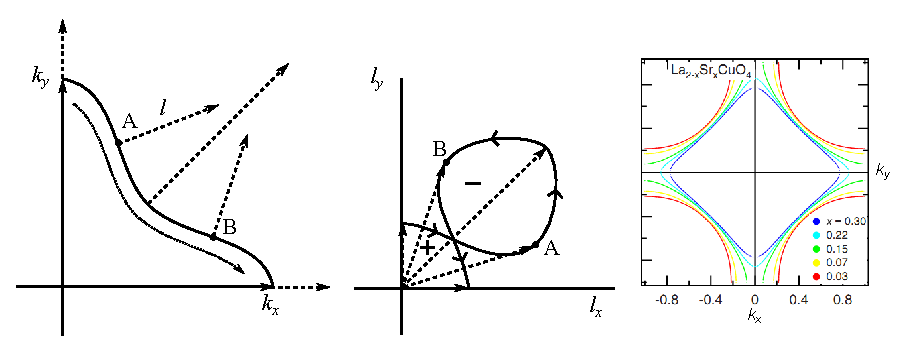
\includegraphics[scale=0.9]{Chapter-Theory/Figures/NegativeCurvatureLSCO/NegativeCurvatureLSCO}
        \caption{Left illustrates a negatively curved Fermi surface with a long mean free path along the $k = (\pi, \pi)$ portion and the integral progressing along the dotted line. Middle shows how the mean free path vector changes along the integral line tracing two loops of opposite direction. Adapted from ref.~\cite{Narduzzo2008}. Right shows the progression of the \ac{BSCO} Fermi surface about the van-Hove singularity. Adapted from ref.~\cite{Kondo2004}.}
        \label{Fig:Theo:NegativeCurvatureLSCO}
    \end{center}
\end{figure}
Narduzzo \etal{} argues that this illustrated scenario is close to what we find in \ac{LSCO} at high doping. Here the mean free path is affected by the anisotropic scattering rate detailed in the introduction section and the proximity of the van-Hove singularity leads to negative curvature in the long flat sides of the Fermi surface as it changes between hole-like and electron-like, as shown for \ac{BSCO} in the right side panel of figure~\ref{Fig:Theo:NegativeCurvatureLSCO}, adapted from ref~\cite{Kondo2004}.

The form of the equations set out originally by Ong~\cite{Ong1991} for a 2D metal derives a relation for the transverse conductivity, $\sigma_{xy}$ from the Boltzmann model are as follows,
\begin{equation}
    \sigma_{xy} = \frac{e^2}{h}\frac{2\phi}{\phi_0} \hspace{8px}\textrm{where}\hspace{8px}\phi = A_l B
\end{equation}
where $A_l$ is the `Stokes' area traced in the centre panel of figure~\ref{Fig:Theo:NegativeCurvatureLSCO} and $\phi$ is the flux through the Stokes area and $\phi_0 = h/e$ is the flux quantum. The Hall coefficient $R_H$ is given by,
\begin{equation}
    R_H = \frac{\sigma_{xy}}{\sigma_{xx}\sigma_{yy}}
\end{equation}
where, assuming symmetric scattering along the $x$ and $y$ directions of the conductivity tensor then,
\begin{equation}
    \sigma_{xx} = \sigma_{yy} = \frac{e^2}{4\pi^2 \hbar} \int^{2\pi}_0 k_F(\theta) l(\theta) d\theta
\end{equation} 
Contributions from isotropic scattering which affect $\sigma_{xy}$ are cancelled in $R_H$, however anisotropic scattering at regions of Fermi surface of particular curvature do contribute to the Hall coefficient.



\section{Magnetoresistance}

\subsection{Fermi liquid theory}



